%-------------------------------------------------------------------------
% Design Project Input/Output Module Description
%-------------------------------------------------------------------------

\clearpage
\section{Accelerometer Input Module}
\label{sec-input-accel}

This input module enables your IoT device to sense the physical
acceleration experienced by your IoT device, perfect for acceleration
measurements for a wide range of applications such as tilt-sensing,
motion, shock, and/or vibration. The ADXL335 3-axis accelerometer you
will use is a micro-electro-mechanical system (MEMS) device -- a device
that combines tightly-coupled electrical and mechanical systems on a
very small scale (micro-meters!). The accelerometer works by measuring
the change in capacitance between fixed plates and a tiny structure
suspended in mid-air by polysilicon springs.  As the device tilts or
experiences motion in the X, Y, and/or Z axes, the suspended structure
deflects and the capacitance on each axis changes. The changes in
capacitance are converted to an output voltage proportional to the
acceleration on that axis, which can be sensed by the Arduino.

A sample circuit and Arduino code is shown below to get you started.
The ADXL335 breakout board is hooked to power and ground, and the data
pins for each axes are wired to analog input pins on the Arduino. The
example code will print calibrated analog
readings from the accelerometer for each axis on the serial monitor, similar to how we
printed the analog reading from the grayscale sensor in Lab~2. After
setting up the circuit and programming the Arduino, open the serial
monitor, place your device on the table, and check the values the
accelerometer is sensing. Then pick up the device, try tilting it, and
see how the values change along the three axes!

\vspace{0.1in}
\begin{minipage}[t]{0.49\tw}

  \vspace{0.1in}
  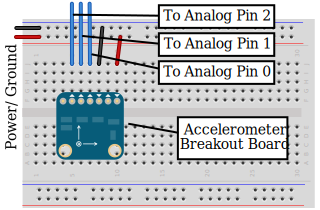
\includegraphics[width=\tw]{input-accel-annotated.svg.pdf}

\end{minipage}
\hfill
\begin{minipage}[t]{0.49\tw}
  \vspace{0.1in}
  \begin{Verbatim}[gobble=3,fontsize=\small]
    int pin_x_accel = 0;
    int pin_y_accel = 1;
    int pin_z_accel = 2;

    // Calibration

    int xmin = 267;
    int xmax = 399;
    int ymin = 272;
    int ymax = 404;
    int zmin = 274;
    int zmax = 412;

    void setup() {
      Serial.begin(9600);
    }

    // Takes 10 readings over 10ms.
    // Returns the average.
    int ReadAxis( int axisPin ) {
      long reading = 0;
      delay(1);
      for(int i = 0; i < 10; ++i)
        reading += analogRead( axisPin );
      return reading / 10;
    }

    void loop() {

      // Read each axis.

      int x_raw = ReadAxis( pin_x_accel );
      int y_raw = ReadAxis( pin_y_accel );
      int z_raw = ReadAxis( pin_z_accel );

      // Scale measurements to calibrated minimum
      // and maximum.

      int x_scaled =
        map( x_raw, x_min, x_max, -1000, 1000 );
      int y_scaled =
        map( y_raw, y_min, y_max, -1000, 1000 );
      int z_scaled =
        map( z_raw, z_min, z_max, -1000, 1000 );

      // Report scaled measurements.

      Serial.print("x: ");
      Serial.print( x_scaled / 1000.0 );
      Serial.print("y: ");
      Serial.print( y_scaled / 1000.0 );
      Serial.print("z: ");
      Serial.print( z_scaled / 1000.0 );
      Serial.println();

      // Wait 500ms before next reading.

      delay(500);
    }
  \end{Verbatim}
\end{minipage}
\vspace{0.1in}

%Questions:
